\todo{bioinformaticka motivacia problemu. blabla. bioinf definicia problemu. Vo
svojej praci sa Dr. Peter Boza PhD., CSc., PanVesmiru, zaobera \ldots, kde
riesi \ldots a odtial pochadza motivacia riesit problem \ldots.}

\section{Definícia problému}

Úlohou bude teda vytvoriť efektívnu dátovú štruktúru, ktorá načíta veľkú sadu
relatívne krátkych reťazcov -- \emph{sequence reads} (pozri časť \ref{sec:sekvenovanie}) a umožní dostatočne rýchlo odpovedať na dotaz \emph{,,vráť tie
reťazce, ktoré obsahujú ako podreťazec reťazec $P$``}, pričom dĺžka reťazca$P$
je dopredu daná. Dôraz budeme klásť ako na rýchlosť odpovedania na query, tak aj
na pamäťovú efektívnosť tejto dátovej štruktúry. Čiže:

\begin{description}
    \item[Vstup] \hfill \\
        Na vstupe pre konštrukciu dátovej štruktúry je prirodzené číslo $k$ -
        dĺžka dotazu a množina $R$, ktorá predstavuje množinu $n$ \emph{readov},
        každý s dĺžkou $l$.
    \item[Výstup] \hfill \\
        Výstupom pre dotaz $p$ je množina $S$ takých \emph{readov} z $R$, ktoré
        obsahujú $p$ ako podreťazec.
\end{description}

V našom kontexte ale platia aj nasledovné veci, ktoré nám riešenie úlohy do
značnej miery uľahčí:

\begin{itemize}
    \item Vieme, že všetky \emph{sequence reads} pochádzajú z nejakého
    spoločného nadslova (sekvenovanej DNA), pričom pri sekvenovaní mohla s
    istou pravdepodobnosťou nastať chyba (pozri časť \ref{sec:sekvenovanie}). Z chýb budeme uvažovať iba substitúciu, ktorej pravdepodobnosť vymedzíme na úroveň $0.1\% - 2\% $. To znamená, že pre každú bázu každého \emph{readu} nastala substitúcia (za nie nutne rôznu bázu) s danou pravdepodobnosťou.
    \item Dĺžka spoločného nadslova sa pohybuje medzi miliónom (dĺžka
    genómu baktérií je niekde na úrovni štyroch miliónov) a jednej
    miliardy (dĺžka genómu človeka je asi tri miliardy báz).
    \item Dĺžky \emph{readov} $l$ sa pohybujú v rozmedzí $100 - 150$ báz.
    \item Pri sekvenovaní sa využíva miera pokrytia (pozri časť \ref{sec:sekvenovanie}) v rozmedzí $10\times$ až $100\times$, z čoho nám v kombinácii s dlžkou spoločného nadslova a dlžkou \emph{readov} vychádza obmedzenie pre počet \emph{readov} na vstupe na 
    $n \in [ 10^5, \frac{2}{3} \cdot 10^9 ]$.
    \item Dĺžku dotazu $p$ budeme uvažovať v rozmedzí $13 -15$. 
    \item A na záver, pri zisťovaní, či $p$ je podreťazcom $r$ budeme testovať
    aj to, či reverzný komplement (pozri časť \ref{sec:formalne_definicie}) $p$ ($revcompl(p)$) nie je podreťazcom $r$ - bude nám stačiť, ak bude túto podmienku spĺňať jeden z nich. \todo{maybe biologicka
    motivacia preco toto?}
\end{itemize}

Cieľom bude dosiahnuť čo najnižsiu pamäťovú zložitosť, pri zachovaní
,,rozumnej`` časovej zložitosti. Očakávaná pamáťová zložitosť bude teda $O(n +
s)$, kde $n$ je počet načítaných \emph{readov} a $s$ je dĺžka spoločného
nadslova. (Triviálnym riešením by bolo $O(n \cdot L)$, kde $L$ je dĺžka
\emph{readu})

\section{Riešenie s použitím hash mapy}
Ako prvé netriviálne riešenie tohto problému sa naskytá použitie hash mapy,
kde kľúčom sú všetky možné hľadané vzorky $p$ (tie generovať vieme,
keďže máme dopredu danú dĺzku $k = |p|$ a pracujeme nad konečnou abecedou) a
hodnota pre daný kľúč by bol zoznam \emph{readov}, ktoré tento \emph{pattern}
obsahujú. Algorimus na generovanie takejto hash mapy by vyzeral naslednovne:

\begin{pseudocode}[label=lst:hash_algorithm,caption={Algoritmus na riešenie
problému zarovnania readov pomocou hash mapy}]
h = HashMap.new

def process(R)
  foreach r : R do
    for i in (0...(|r| - k + 1)) do
      t = r[i, k]
      if not h.has_key?(t)
        h[t] = LinkedList.new
      end
        
      h[t].append(r)
    end 
  end
end

def find_reads(p)
  return (h[p].append(h[revcompl(p)]))
end
\end{pseudocode}

Pre každý \emph{read} $r$ zo zoznamu \emph{readov} $R$ vygerujeme všetky jeho
podreťazce dĺžky $k$ a tie použijeme ako kľúče do hash mapy, pomocou ktorých
tento \emph{read} zaindexujeme jeho pridaním do spájaného zozanmu.

Hľadanie vzorky $p$ potom prebieha tak, že vrátime zreťazené spájané
zoznamy pre $p$ a reverzný komplement $p$.

\begin{example}
    Príklad hash mapy pre množinu \emph{readov} $$S = \{ACTTT, CTTAT, TTTAT,
    AAACT, ACTGA\}$$.
    \begin{figure}[h]
        \centering
        \includegraphics[width=6cm]{hash_map}
        \caption{Hash mapa}
        \label{fig:hash_map}
    \end{figure}
    \\
    Pre vzorku napr. $TTT$ by teda bola výsledkom množina \emph{readov} $R =
    \{ACTTT, CTTAT, AAACT\}$.
\end{example}

Vyhľadávanie vzorky prebieha v konštantnom čase, no pamäťová uložitosť tohto
riešenia ale nie je ani zďaleka optimálna, v najhoršom prípade až $O(n \cdot
l)$. Existuje množstvo zlepšení, napríklad:

\begin{itemize}
    \item miesto celých \emph{readov} nám stačí si v spájanom zozname
    pamätať len indexy daných readov
    \item kľúče možno komprimovať napríklad nasledovným spôsobom: pre znaky
    tvoriace kľúče vytvoríme nasledovné kódovanie: $A = 00$, $C = 01$, $T = 10$,
    $G = 11$ a pomocou neho zakódujeme celý kľúč, čím dostaneme bitový vektor
    (v našom príklade uvedenom vyššie 6-bitový), ktorý sa už komprimuje oveľa
    jednoduchšie (napríklad ako celé číslo).
\end{itemize}

\todo{dalsie zlepsenia?}

\section{Riešenie s použitím GkArray}

\section{Porovnanie}